\documentclass[,man]{apa6}
\usepackage{lmodern}
\usepackage{amssymb,amsmath}
\usepackage{ifxetex,ifluatex}
\usepackage{fixltx2e} % provides \textsubscript
\ifnum 0\ifxetex 1\fi\ifluatex 1\fi=0 % if pdftex
  \usepackage[T1]{fontenc}
  \usepackage[utf8]{inputenc}
\else % if luatex or xelatex
  \ifxetex
    \usepackage{mathspec}
  \else
    \usepackage{fontspec}
  \fi
  \defaultfontfeatures{Ligatures=TeX,Scale=MatchLowercase}
\fi
% use upquote if available, for straight quotes in verbatim environments
\IfFileExists{upquote.sty}{\usepackage{upquote}}{}
% use microtype if available
\IfFileExists{microtype.sty}{%
\usepackage{microtype}
\UseMicrotypeSet[protrusion]{basicmath} % disable protrusion for tt fonts
}{}
\usepackage{hyperref}
\hypersetup{unicode=true,
            pdftitle={nStreams Analysis},
            pdfauthor={Charles J. H. Ludowici~\& Alex O. Holcombe},
            pdfkeywords={keywords},
            pdfborder={0 0 0},
            breaklinks=true}
\urlstyle{same}  % don't use monospace font for urls
\usepackage{graphicx,grffile}
\makeatletter
\def\maxwidth{\ifdim\Gin@nat@width>\linewidth\linewidth\else\Gin@nat@width\fi}
\def\maxheight{\ifdim\Gin@nat@height>\textheight\textheight\else\Gin@nat@height\fi}
\makeatother
% Scale images if necessary, so that they will not overflow the page
% margins by default, and it is still possible to overwrite the defaults
% using explicit options in \includegraphics[width, height, ...]{}
\setkeys{Gin}{width=\maxwidth,height=\maxheight,keepaspectratio}
\IfFileExists{parskip.sty}{%
\usepackage{parskip}
}{% else
\setlength{\parindent}{0pt}
\setlength{\parskip}{6pt plus 2pt minus 1pt}
}
\setlength{\emergencystretch}{3em}  % prevent overfull lines
\providecommand{\tightlist}{%
  \setlength{\itemsep}{0pt}\setlength{\parskip}{0pt}}
\setcounter{secnumdepth}{0}
% Redefines (sub)paragraphs to behave more like sections
\ifx\paragraph\undefined\else
\let\oldparagraph\paragraph
\renewcommand{\paragraph}[1]{\oldparagraph{#1}\mbox{}}
\fi
\ifx\subparagraph\undefined\else
\let\oldsubparagraph\subparagraph
\renewcommand{\subparagraph}[1]{\oldsubparagraph{#1}\mbox{}}
\fi

%%% Use protect on footnotes to avoid problems with footnotes in titles
\let\rmarkdownfootnote\footnote%
\def\footnote{\protect\rmarkdownfootnote}


  \title{nStreams Analysis}
    \author{Charles J. H. Ludowici\textsuperscript{1}~\& Alex O.
Holcombe\textsuperscript{1}}
      \date{5/18/2017}

\shorttitle{SHORTTITLE}
\authornote{Add complete departmental affiliations for each author here. Each new line herein must be indented, like this line.

Enter author note here.


Correspondence concerning this article should be addressed to Charles J. H. Ludowici, USYD. E-mail: charles.ludowici@sydney.edu.au}
\affiliation{
\vspace{0.5cm}
\textsuperscript{1} The University of Sydney}
\abstract{Enter abstract here. Each new line herein must be indented, like this line.
}
\keywords{keywords\newline\indent Word count: X}
\usepackage{csquotes}
\usepackage{upgreek}
\captionsetup{font=singlespacing,justification=justified}

\usepackage{longtable}
\usepackage{lscape}
\usepackage{multirow}
\usepackage{tabularx}
\usepackage[flushleft]{threeparttable}
\usepackage{threeparttablex}

\newenvironment{lltable}{\begin{landscape}\begin{center}\begin{ThreePartTable}}{\end{ThreePartTable}\end{center}\end{landscape}}

\makeatletter
\newcommand\LastLTentrywidth{1em}
\newlength\longtablewidth
\setlength{\longtablewidth}{1in}
\newcommand{\getlongtablewidth}{\begingroup \ifcsname LT@\roman{LT@tables}\endcsname \global\longtablewidth=0pt \renewcommand{\LT@entry}[2]{\global\advance\longtablewidth by ##2\relax\gdef\LastLTentrywidth{##2}}\@nameuse{LT@\roman{LT@tables}} \fi \endgroup}


\DeclareDelayedFloatFlavor{ThreePartTable}{table}
\DeclareDelayedFloatFlavor{lltable}{table}
\makeatletter
\renewcommand{\efloat@iwrite}[1]{\expandafter\immediate\expandafter\protected@write\csname efloat@post#1\endcsname{}}
\makeatother
\usepackage{lineno}

\linenumbers

\begin{document}
\maketitle

\begin{center}\rule{0.5\linewidth}{\linethickness}\end{center}

\begin{verbatim}
## 
##  Paired t-test
## 
## data:  latency$eightStreams and latency$twoStreams
## t = 6.429, df = 9, p-value = 0.0001211
## alternative hypothesis: true difference in means is not equal to 0
## 95 percent confidence interval:
##  26.57040 55.42028
## sample estimates:
## mean of the differences 
##                40.99534
\end{verbatim}

\section{Latency Analyses}\label{latency-analyses}

\begin{verbatim}
## [1] 242.5299
\end{verbatim}

\begin{verbatim}
## [1] 484.9676
\end{verbatim}

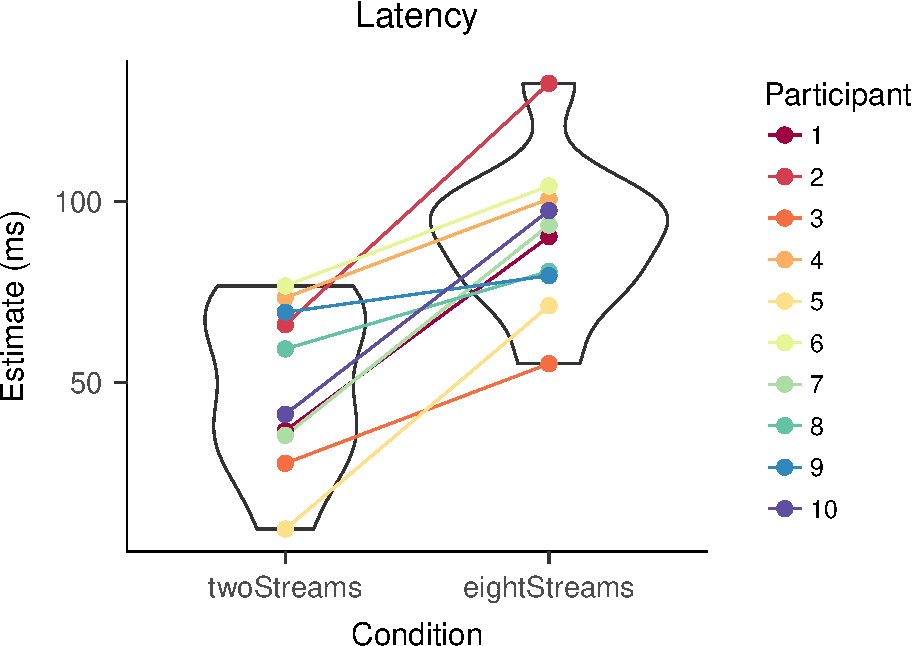
\includegraphics{nStreams_Bayesian_files/figure-latex/unnamed-chunk-3-1.pdf}
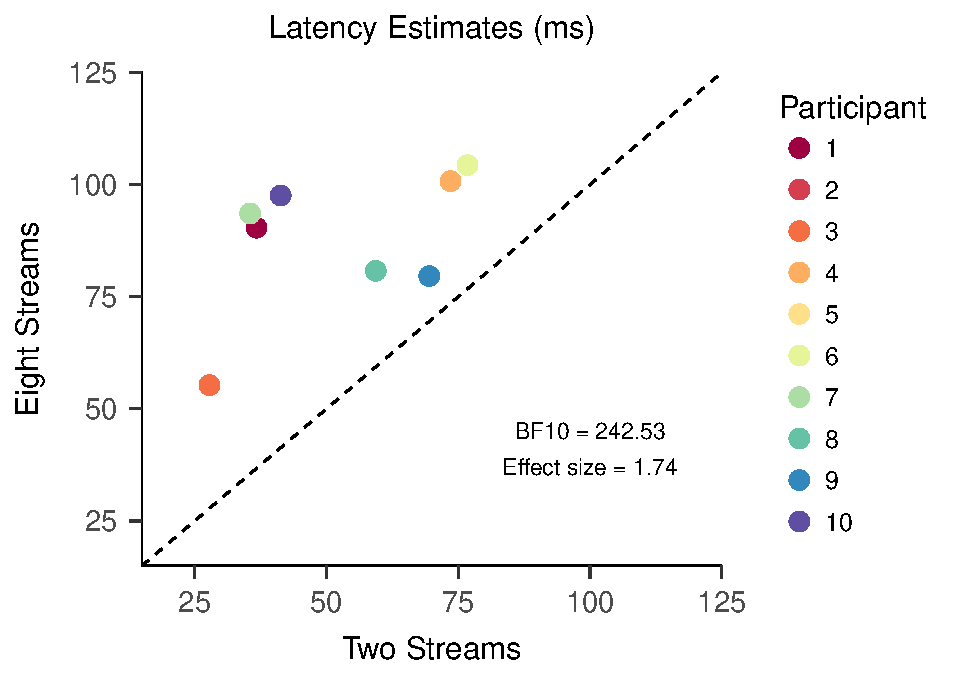
\includegraphics{nStreams_Bayesian_files/figure-latex/unnamed-chunk-3-2.pdf}

\section{Precision Analysis}\label{precision-analysis}

\begin{verbatim}
## [1] 41.11253
\end{verbatim}

\begin{verbatim}
## [1] 0.09697909
\end{verbatim}

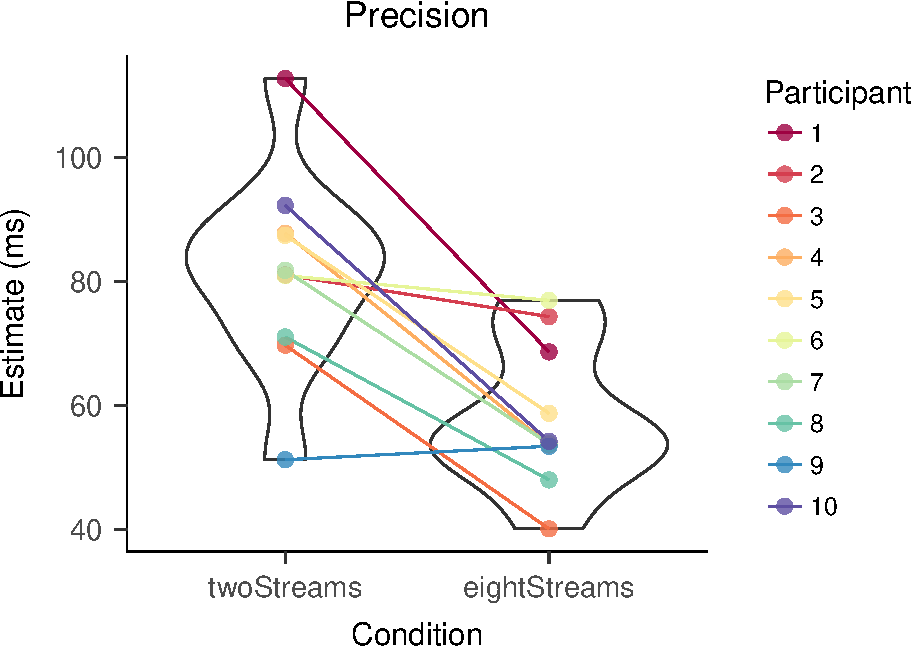
\includegraphics{nStreams_Bayesian_files/figure-latex/unnamed-chunk-4-1.pdf}
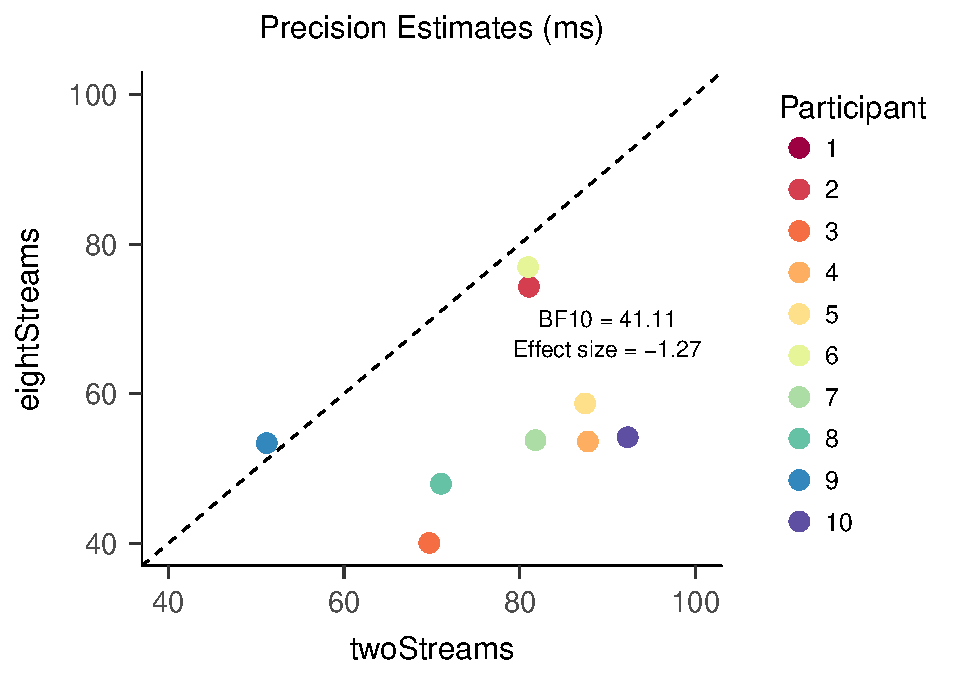
\includegraphics{nStreams_Bayesian_files/figure-latex/unnamed-chunk-4-2.pdf}

\section{Efficacy Analysis}\label{efficacy-analysis}

\begin{verbatim}
## [1] 0.3755812
\end{verbatim}

\begin{verbatim}
## [1] 0.5468815
\end{verbatim}

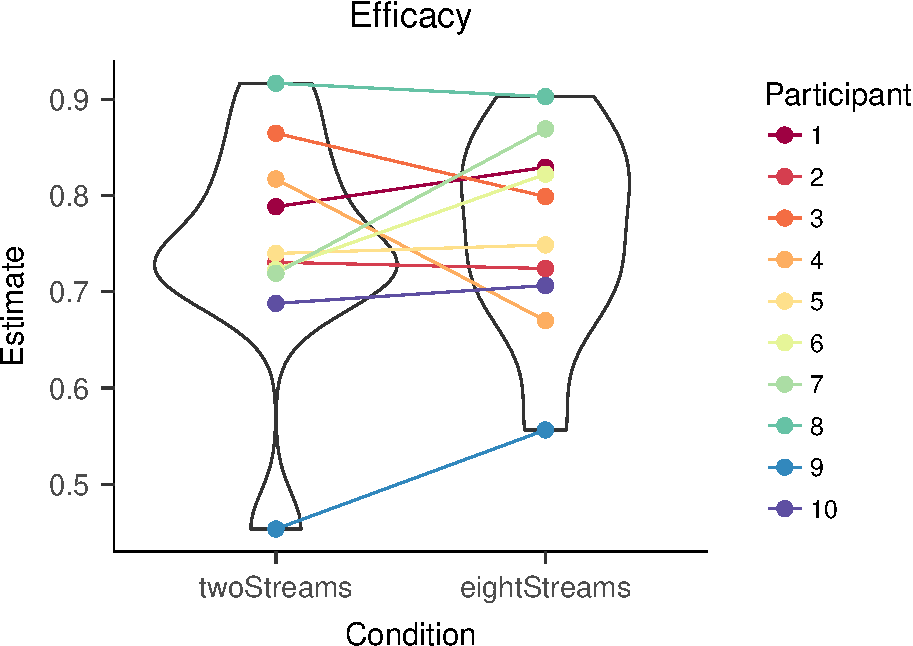
\includegraphics{nStreams_Bayesian_files/figure-latex/unnamed-chunk-5-1.pdf}
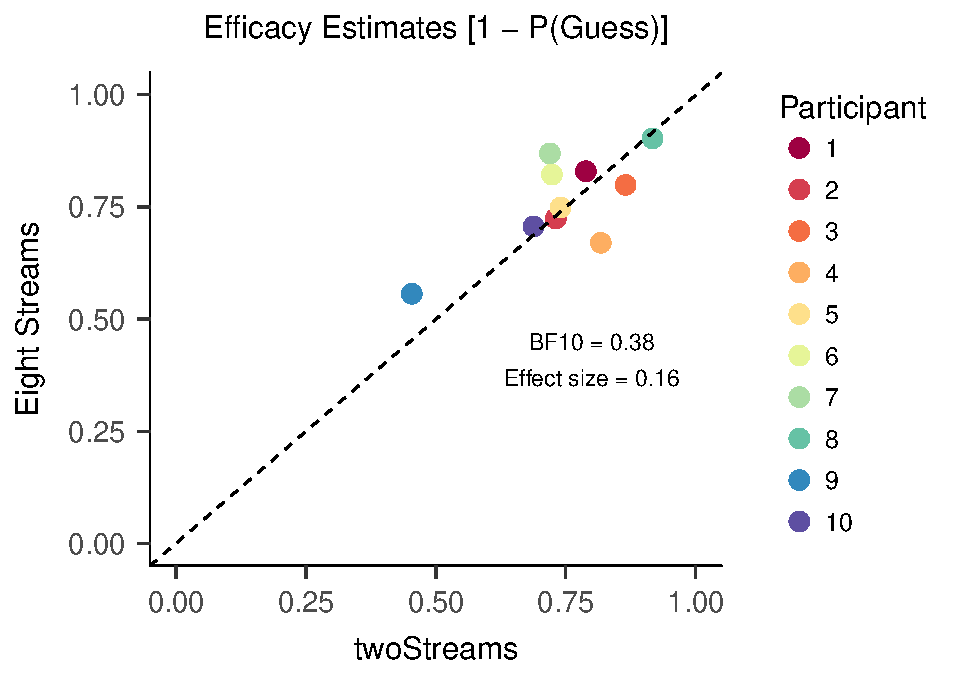
\includegraphics{nStreams_Bayesian_files/figure-latex/unnamed-chunk-5-2.pdf}

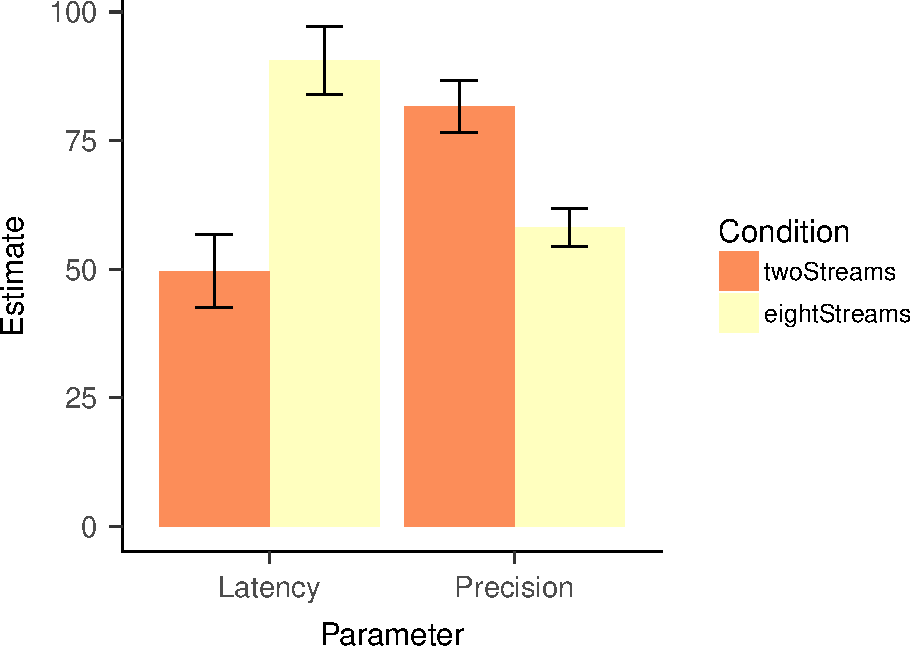
\includegraphics{nStreams_Bayesian_files/figure-latex/unnamed-chunk-6-1.pdf}
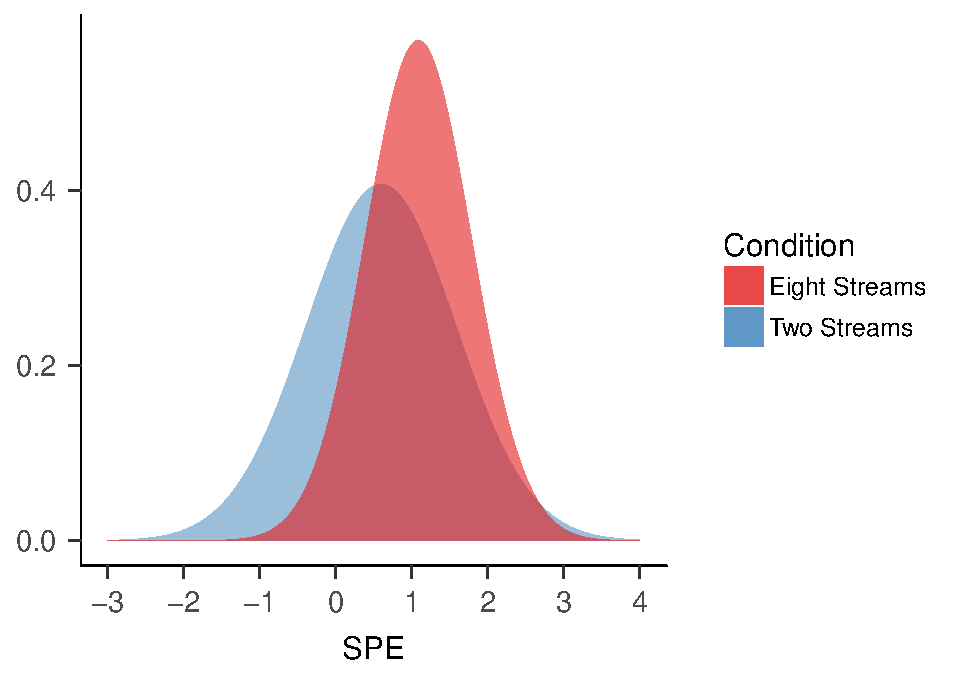
\includegraphics{nStreams_Bayesian_files/figure-latex/unnamed-chunk-6-2.pdf}

\begin{verbatim}
## Warning: Removed 1 rows containing missing values (geom_point).
\end{verbatim}

\begin{verbatim}
## Warning: Removed 2 rows containing missing values (geom_point).
\end{verbatim}


\end{document}
